\documentclass[a4paper]{article}
\usepackage{ctex}
\usepackage{enumitem}
\usepackage{fancyhdr}
\usepackage{amsmath}
\usepackage{parskip}
\usepackage{float}
\usepackage{listings}
\usepackage{hyperref}
\usepackage{xcolor}

\setlength{\parskip}{6pt}

\pagestyle{headings}

\begin{document}
\title{四位加法器}
\author{梁业升 2019010547(计03)}

\maketitle

% GitHub styles
\definecolor{keyword}{HTML}{CF222E}
\definecolor{comment}{HTML}{6E7781}
\definecolor{string}{HTML}{0A3069}

\lstset{
    commentstyle=\color{comment},
    keywordstyle=\color{keyword},
    stringstyle=\color{string},
    basicstyle=\ttfamily\small,
    breakatwhitespace=false,
    breaklines=true,
    captionpos=b,
    keepspaces=true,
    showspaces=false,
    showstringspaces=false,
    showtabs=false,
}


\section{实现}
\subsection{逐次进位}
\subsubsection{一位全加器}

\begin{lstlisting}[language=vhdl]
library ieee;
use ieee.std_logic_1164.all;
use ieee.std_logic_arith.all;
use ieee.std_logic_unsigned.all;

entity fa1 is
    port(
        a, b, c1: in std_logic; -- 输入信号
        s, c2: out std_logic    -- 输出信号
    );
end fa1;

architecture add of fa1 is
begin
    process(a, b, c1)
    begin
        s <= a xor b xor c1;
        c2 <= (a and b) or (a and c1) or (b and c1);
    end process;
end add;
\end{lstlisting}

工作原理:1位加法器元件,传入两个操作数\texttt{a},\texttt{b}和进位信号\texttt{c1},根据逻辑表达式输出结果\texttt{s}和进位信号\texttt{c2}。

\subsubsection{四位全加器}

\begin{lstlisting}[language=vhdl]
library ieee;
use ieee.std_logic_1164.all;
use ieee.std_logic_arith.all;
use ieee.std_logic_unsigned.all;

entity adder is
    port(
        a, b: in std_logic_vector(3 downto 0); -- 输入信号
        c1: in std_logic;                      -- 进位信号
        s: out std_logic_vector(3 downto 0);   -- 输出结果
        c2: out std_logic                      -- 进位信号
    );
end adder;

architecture add of adder is
    component fa1
        port(
            a, b, c1: in std_logic;
            s, c2: out std_logic
        );
    end component;
    signal c: std_logic_vector(2 downto 0);
begin
    f0:fa1 port map (a(0), b(0), c1, s(0), c(0));   -- 映射
    f1:fa1 port map (a(1), b(1), c(0), s(1), c(1));
    f2:fa1 port map (a(2), b(2), c(1), s(2), c(2));
    f3:fa1 port map (a(3), b(3), c(2), s(3), c2);
end add;
\end{lstlisting}

工作原理:使用元件例化,级联构造四位加法器。

\subsection{超前进位}
\subsubsection{一位全加器}

\begin{lstlisting}[language=vhdl]
library ieee;
use ieee.std_logic_1164.all;
use ieee.std_logic_arith.all;
use ieee.std_logic_unsigned.all;

entity fa1 is
    port(
        a, b, c1: in std_logic; -- 输入信号
        s, c2: out std_logic;   -- 输出信号
        p, g: buffer std_logic  -- 中间结果
    );
end fa1;

architecture add of fa1 is
begin
    process(a, b)
    begin
        p <= a xor b;
        g <= a and b;
    end process;
    
    process (c1, p, g)
    begin
        s <= p xor c1;
        c2 <= (p and c1) or g;
    end process;
end add;
\end{lstlisting}

工作原理:1位加法器元件,在之前版本的基础上增加了中间信号\texttt{p}和\texttt{g}用于超前进位。

\subsubsection{四位全加器}

\begin{lstlisting}[language=vhdl]
library ieee;
use ieee.std_logic_1164.all;
use ieee.std_logic_arith.all;
use ieee.std_logic_unsigned.all;

entity adder is
    port(
        a, b: in std_logic_vector(3 downto 0); -- 输入信号
        c1: in std_logic;                      -- 进位信号
        s: out std_logic_vector(3 downto 0);   -- 输出结果
        c2: out std_logic                      -- 进位信号
    );
end adder;

architecture add of adder is
    component fa1
        port(
            a, b, c1: in std_logic;
            s, c2: out std_logic;
            p, g: buffer std_logic
        );
    end component;
    signal c: std_logic_vector(2 downto 0);
    signal p, g: std_logic_vector(3 downto 0); -- 超前进位信号
begin
    f0:fa1 port map (a=>a(0), b=>b(0), c1=>c1, s=>s(0), p=>p(0), g=>g(0));
    f1:fa1 port map (a=>a(1), b=>b(1), c1=>c(0), s=>s(1), p=>p(1), g=>g(1));
    f2:fa1 port map (a=>a(2), b=>b(2), c1=>c(1), s=>s(2), p=>p(2), g=>g(2));
    f3:fa1 port map (a=>a(3), b=>b(3), c1=>c(2), s=>s(3), p=>p(3), g=>g(3));
    
    process(p, g)
    begin
            c(0) <= g(0) or (p(0) and c1);
            c(1) <= g(1) or (p(1) and g(0)) or (p(1) and p(0) and c1);
            c(2) <= g(2) or (p(2) and g(1)) or (p(2) and p(1) and g(0)) or (p(2) and p(1) and p(0) and c1);
            c2 <= g(3) or (p(3) and g(2)) or (p(3) and p(2) and g(1)) or (p(3) and p(2) and p(1) and g(0)) or (p(3) and p(2) and p(1) and p(0) and c1);
    end process;
end add;
\end{lstlisting}

工作原理:使用元件例化,利用每个一位加法器的\texttt{p}、\texttt{g}信号进行超前进位。

\section{实验结果}

\subsection{仿真结果}

\begin{figure}[H]
    \centering
    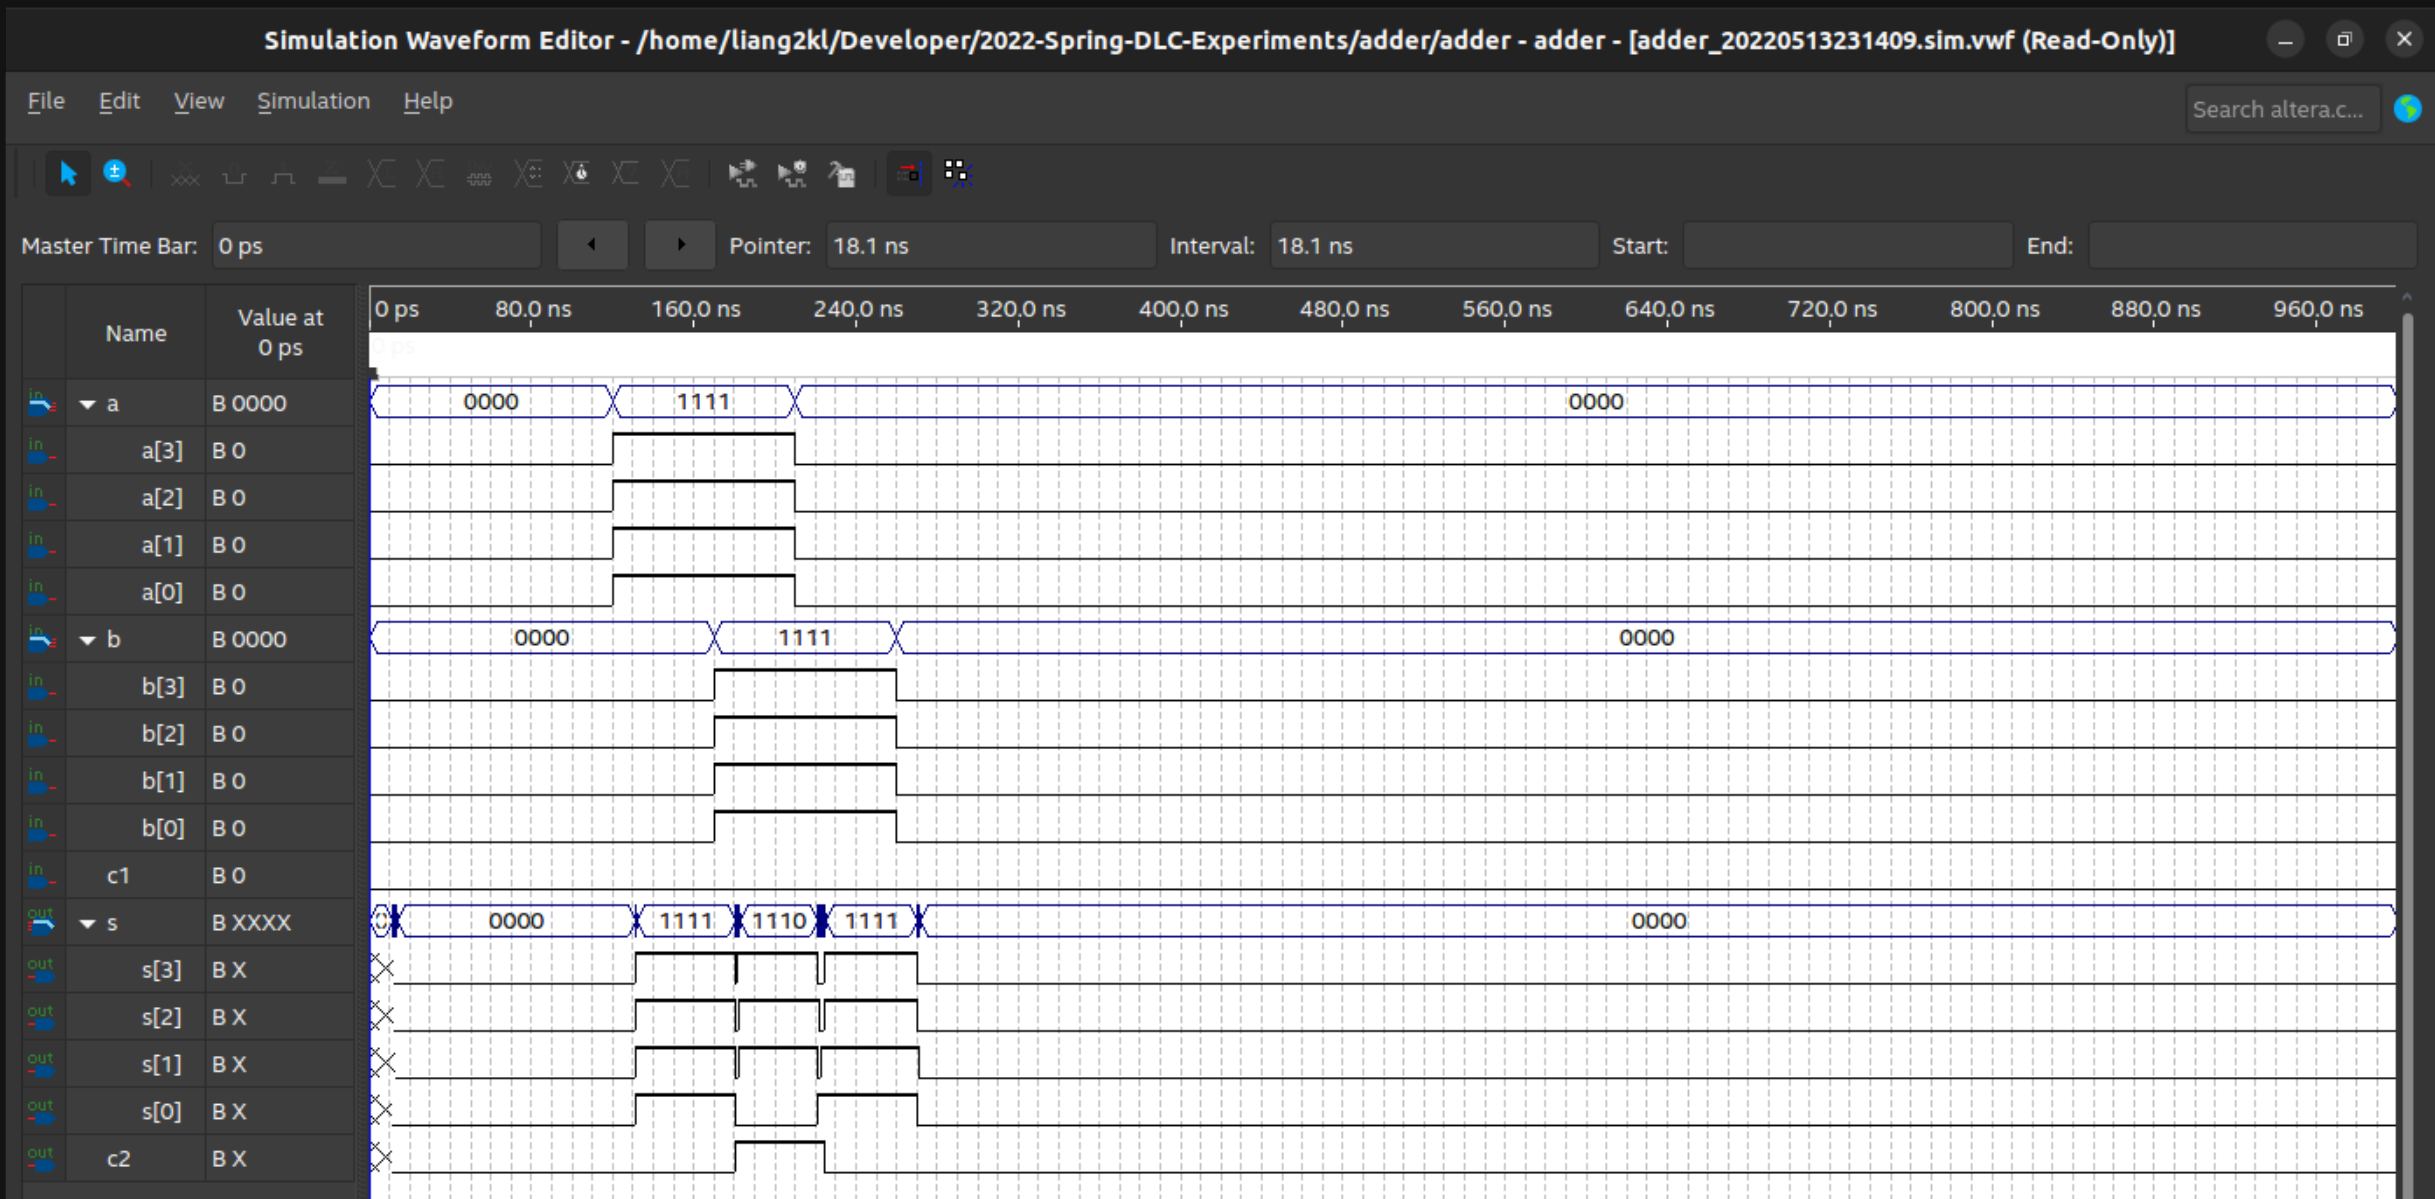
\includegraphics[width=1\textwidth]{./assets/simulation-1.png}
    \caption{逐次进位仿真结果}
\end{figure}

\begin{figure}[H]
    \centering
    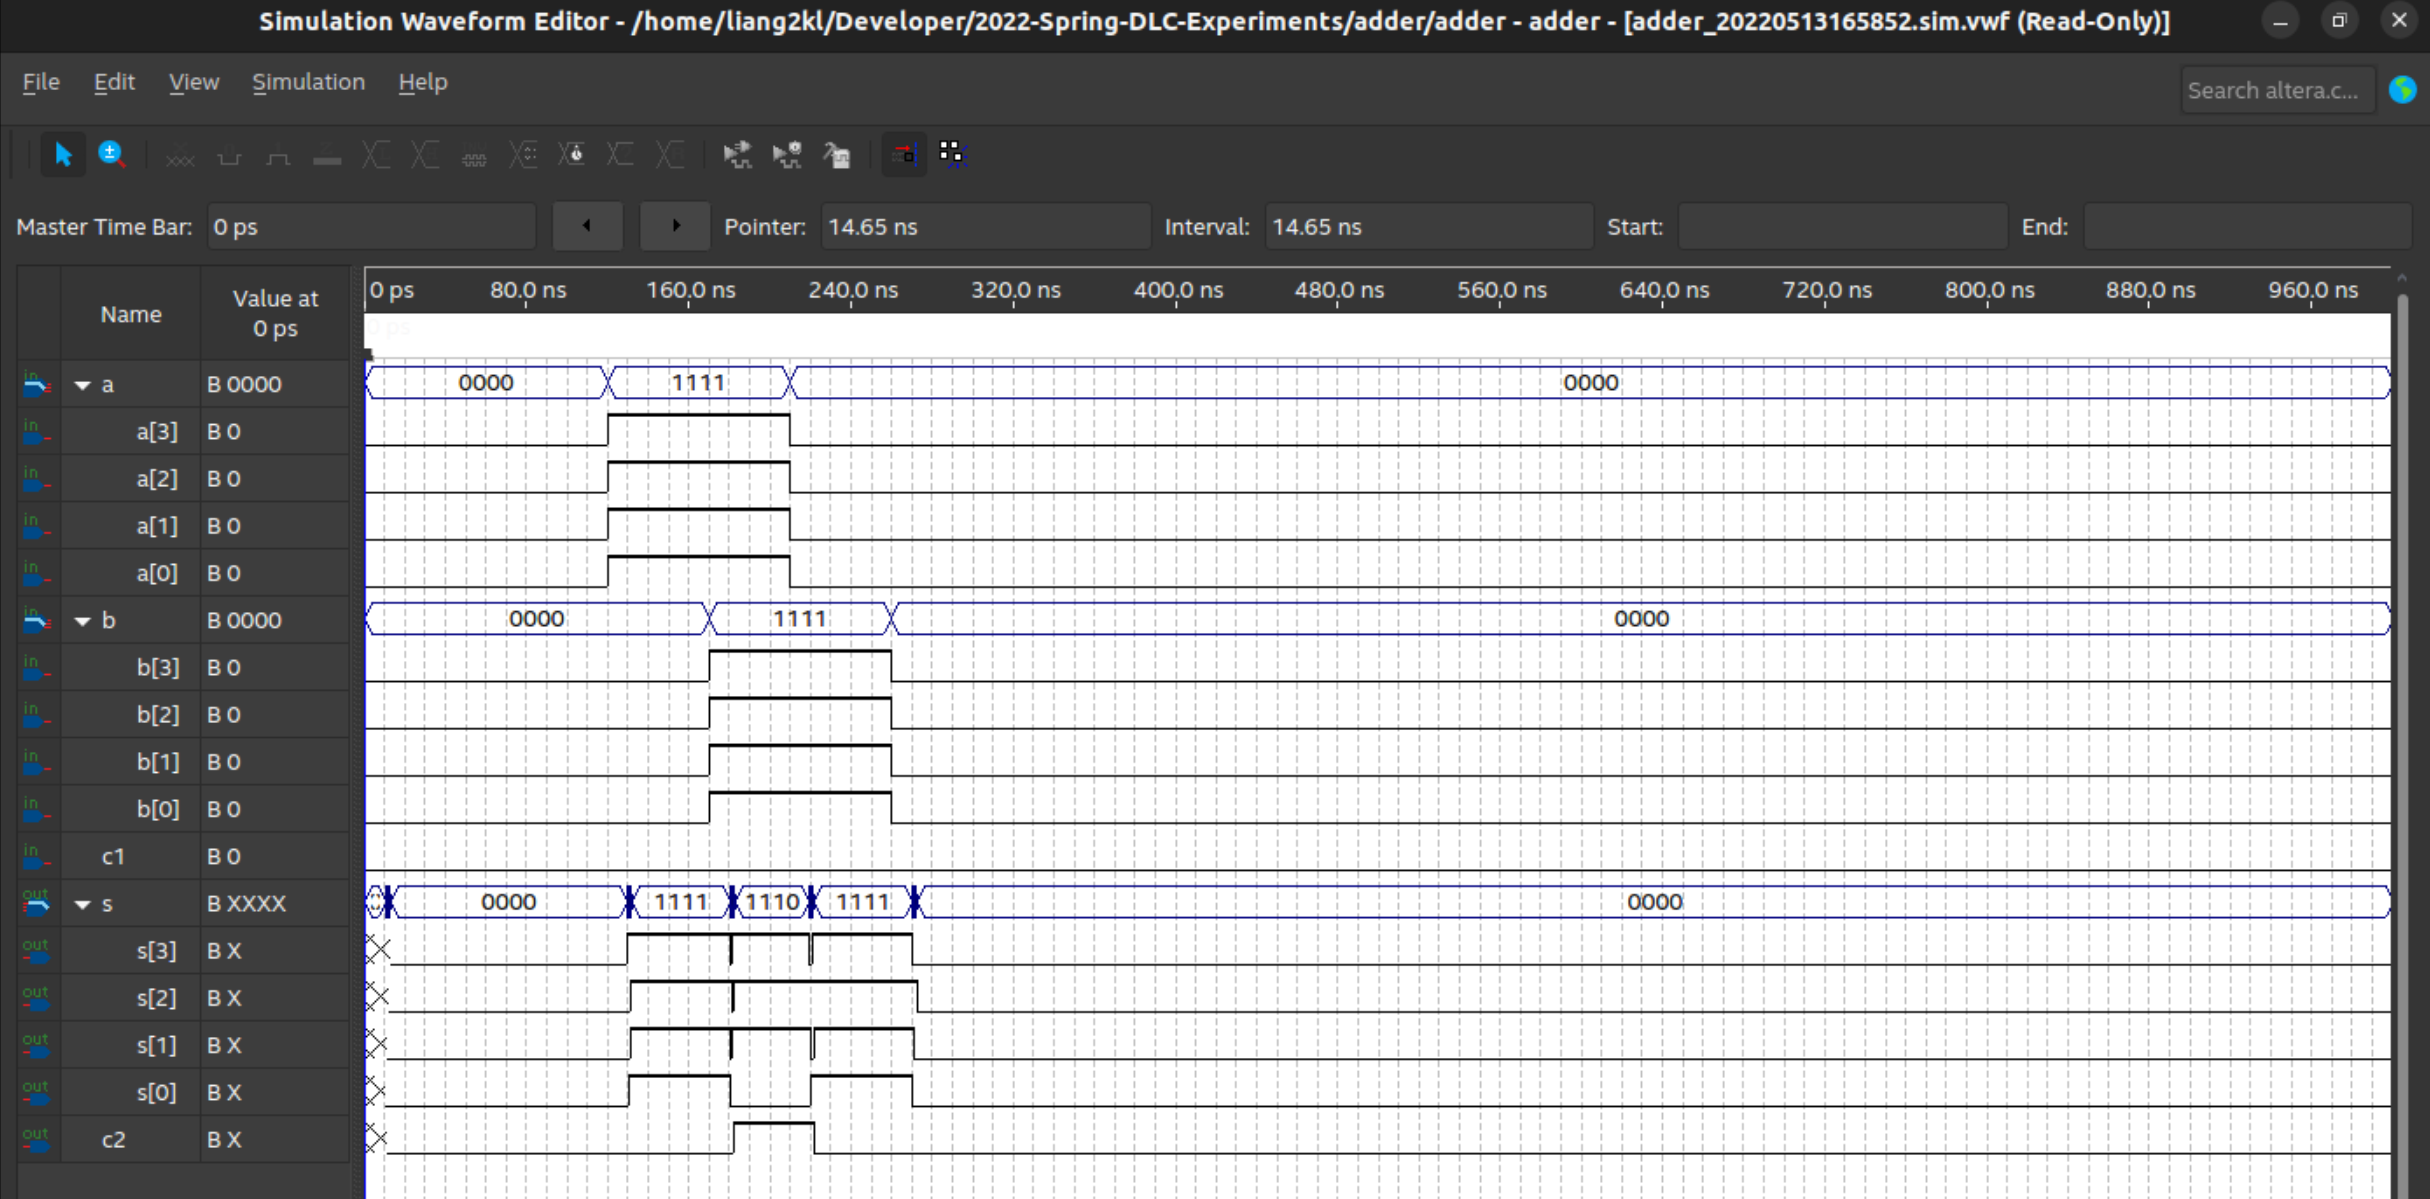
\includegraphics[width=1\textwidth]{./assets/simulation-2.png}
    \caption{超前进位仿真结果}
\end{figure}

因位数不高,二者时延差别不大。

\subsection{实际操作结果}

加法器能够正常处理输入、输出以及进位。

\section{实验总结}

由于有了第一次实验的基础,本次实验代码编写进展比较顺利,没有遇到较大的问题。在仿真软件的环境配置上花了不少时间,不过最终总算是完成了,也积累了相关的经验。

\end{document}
